\documentclass[tikz,border=5mm]{standalone}
\usetikzlibrary{calc}
\begin{document}
	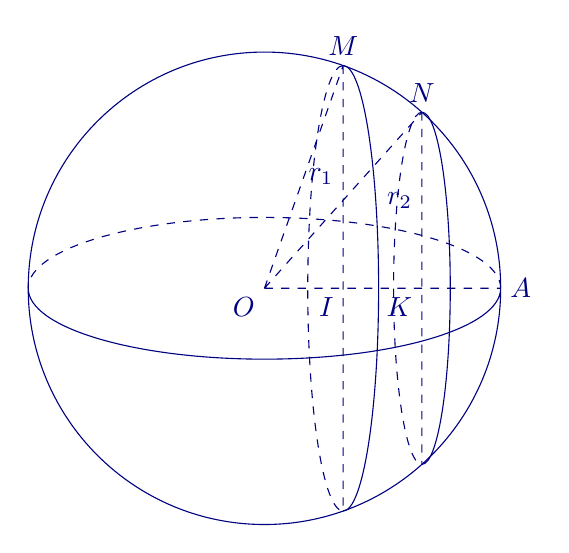
\begin{tikzpicture}[scale=3,blue!50!black]
		\pgfmathsetmacro{\phione}{acos(1/3)}
		\pgfmathsetmacro{\phitwo}{acos(2/3)}
		\pgfmathsetmacro{\m}{sin(\phione)}
		\pgfmathsetmacro{\n}{sin(\phitwo)}
		\path
		(0,0) coordinate (O) node[below left]{$O$}
		--(1,0) coordinate (A) node[right]{$A$}
		(0:1/3) coordinate (I)node[below left]{$I$}
		(0:2/3) coordinate (K)node[below left]{$K$}
		(\phione:1) coordinate (M)node[above] {$M$}
		(\phitwo:1) coordinate(N)node[above] {$N$};
		\draw[dashed]
		(O)--(M) (O)--(N) (O)--(A)
		(M)--(I)node[midway,left]{$r_1$}--([turn]0:\m)
		(N)--(K)node[midway,left]{$r_2$}--([turn]0:\n)
		(A) arc(0:180:1 and .3);
		\draw (M) arc(90:-90: .15 and {\m});
		\draw (N) arc(90:-90: .12 and {\n} );
		\draw[dashed] (M) arc(90:270: .15 and {\m});
		\draw[dashed] (N) arc(90:270: .12 and {\n} );
		\draw
		(A) arc(0:-180:1 and .3)
		(O) circle(1);
	\end{tikzpicture}
\end{document}